\documentclass[11pt]{article}

\usepackage[margin=1in]{geometry}
\usepackage{graphicx}
\usepackage{float}
\usepackage{titlesec}
\usepackage{caption}

\titleformat{\section}{\large\bfseries}{}{0em}{}
\captionsetup[figure]{font=small,labelfont=bf}

\begin{document}

\begin{center}
    {\Large \textbf{Assignment 2 Report}}\\[6pt]
    Vinaykumar Reddy Junuthula
\end{center}

\vspace{0.5em}

\section*{System Architecture}

The experiments were conducted on the Lonestar6 supercomputer. Each compute node consists of AMD EPYC 7763 processors with 64 cores per socket and two sockets per node, resulting in 128 cores per node. The architecture is x86\_64 with two NUMA nodes per system. Each core has L1 and L2 caches, while a large shared L3 cache is available across cores. The system provides high memory bandwidth and supports large-scale parallel execution using MPI, making it suitable for evaluating communication-intensive parallel programs.

\section*{Experiment Setup}

Two execution models were implemented using MPI: a producer-consumer model and a work-pool model.

In the producer-consumer model, rank 0 acts as a centralized broker managing a bounded buffer. Producers generate work messages and send them to the broker, while consumers request work from it. This design introduces centralized coordination and makes the broker a critical communication point.

In the work-pool model, all processes act as both producers and consumers. Each process sends work messages to random processes and consumes incoming work directly, eliminating centralized coordination and distributing communication across all ranks.

Each program was executed with 4, 8, 12, and 16 processes. For each configuration, five runs were performed for 120 seconds. Throughput was computed as the number of messages consumed per second. The average throughput across the five runs is shown in Figure 1, with error bars representing the minimum and maximum values observed for each configuration.

\section*{Performance Results}

\begin{figure}[H]
    \centering
    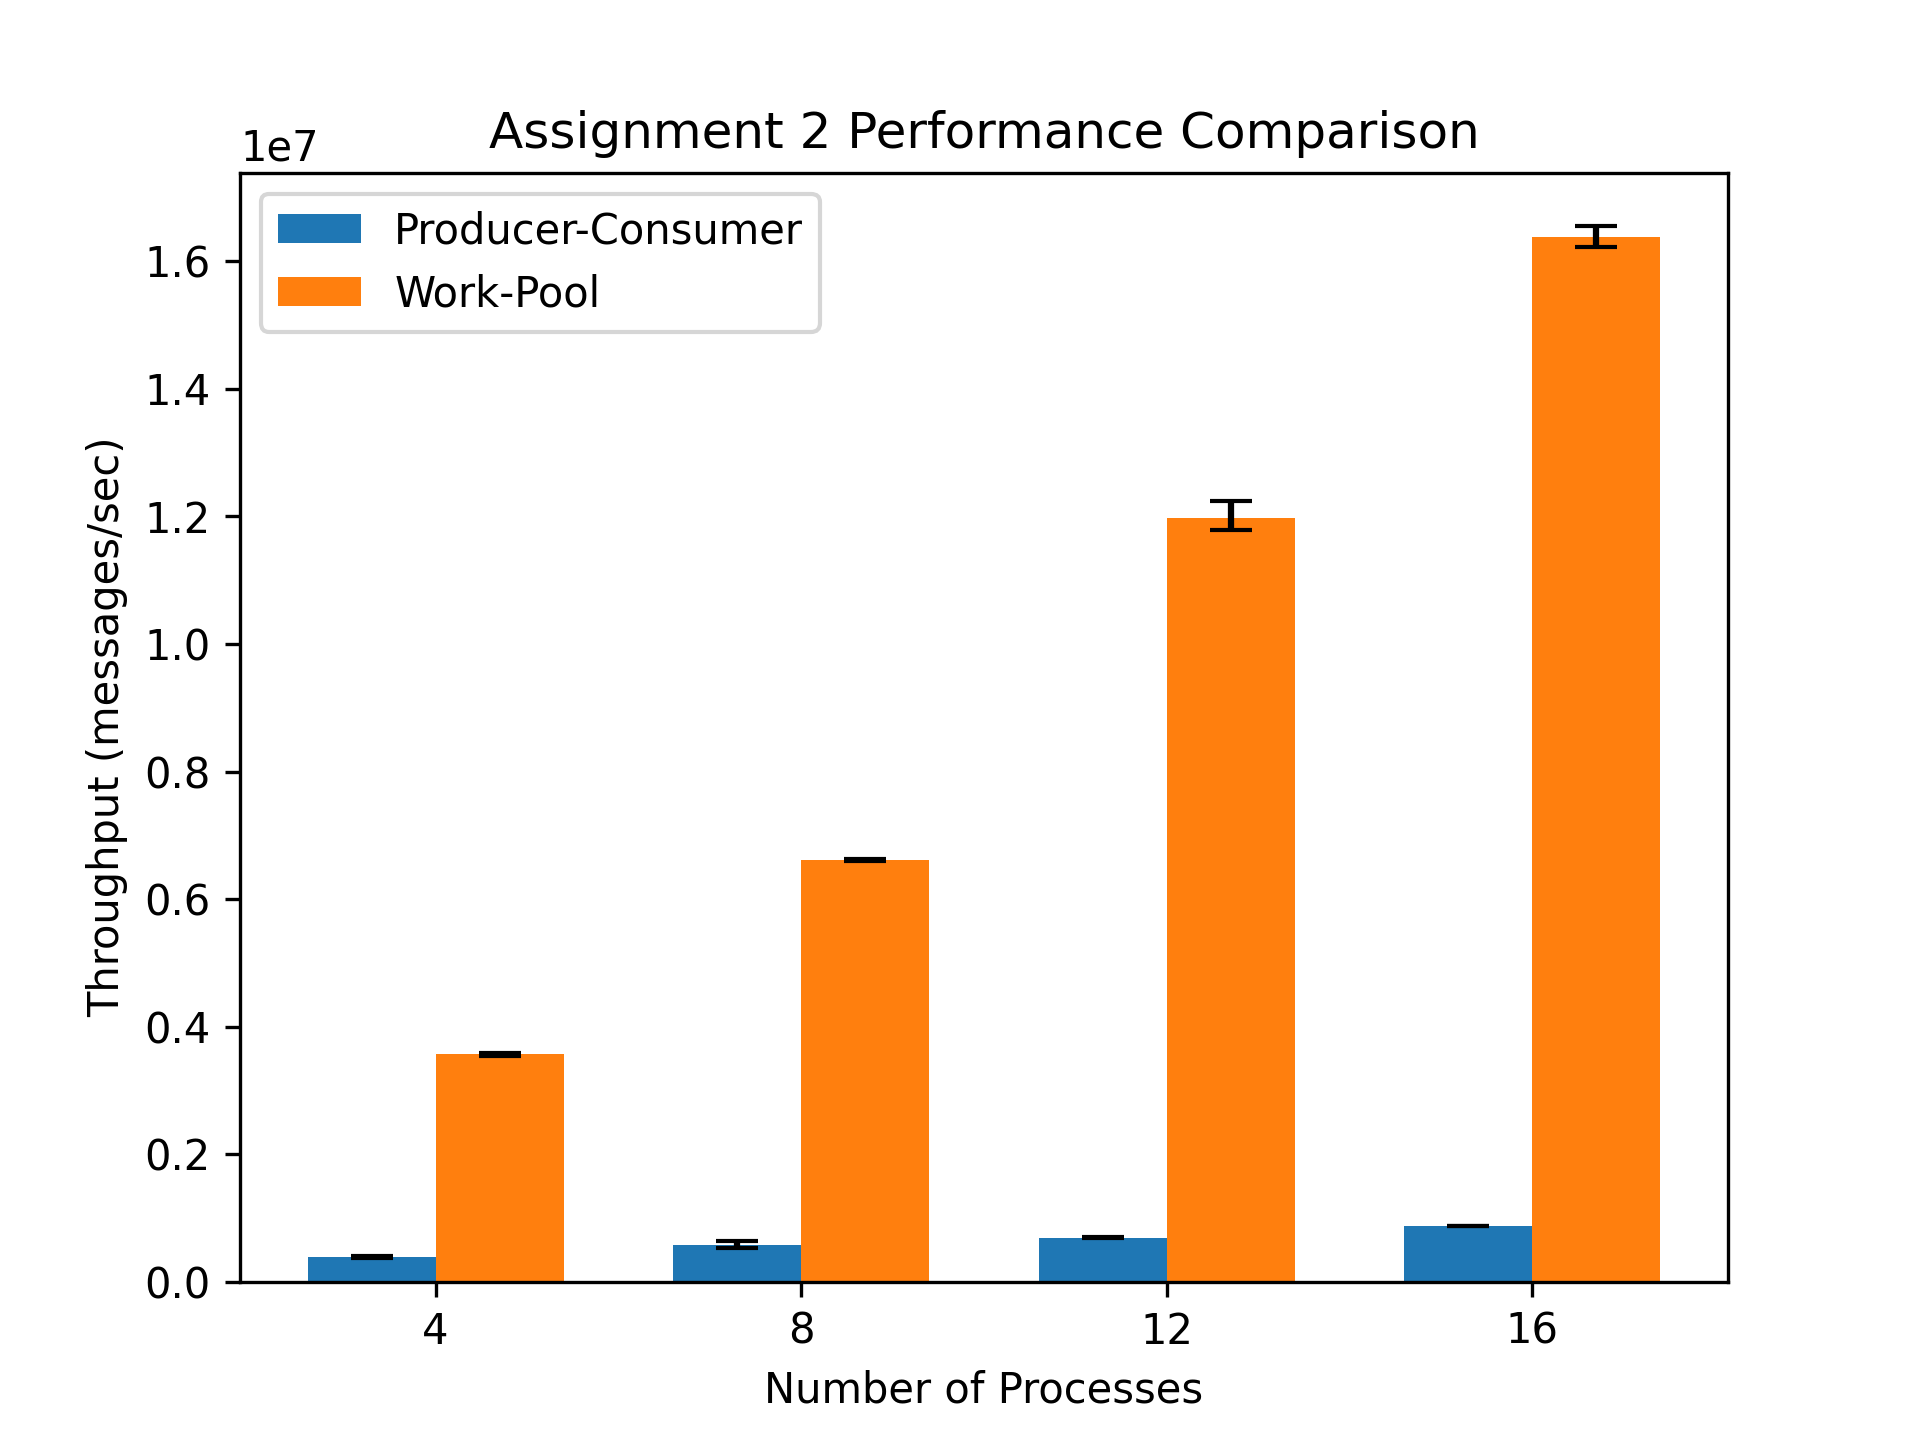
\includegraphics[width=0.82\textwidth]{chart.png}
    \caption{Throughput comparison of Producer-Consumer and Work-Pool models. Each bar shows the average throughput across five runs, and the error bars represent the minimum and maximum throughput values.}
\end{figure}

\section*{Observations}

The results show that throughput increases as the number of processes increases for both execution models. However, the work-pool model significantly outperforms the producer-consumer model at all process counts.

At 4 processes, the producer-consumer model achieves roughly 0.39 million messages per second, while the work-pool model achieves about 3.57 million messages per second. At 16 processes, the producer-consumer model reaches about 0.87 million messages per second, whereas the work-pool model reaches approximately 16.38 million messages per second. This demonstrates that the performance gap becomes even more pronounced as the process count increases.

The producer-consumer model scales more slowly because rank 0 acts as a centralized broker and becomes a communication bottleneck. As more producers and consumers are added, the broker must handle more requests and more message traffic, which limits overall throughput and reduces scalability.

In contrast, the work-pool model distributes communication across all processes, eliminating the single-point bottleneck present in the producer-consumer design. This allows more parallel message exchanges to occur simultaneously and results in substantially higher throughput.

The error bars indicate some variability across runs, which can be attributed to communication overhead, runtime scheduling differences, and system-level noise. Even with this variation, the overall trend is very clear: the decentralized work-pool model provides much better performance and scalability than the centralized producer-consumer model.

\end{document}
